\documentclass[12pt]{article}
%\renewcommand\normalsize{\fontsize{10pt}{12pt}\selectfont}
\usepackage{graphicx} % Required for inserting images
\usepackage[left=2cm,right=2cm,top=2cm,bottom=1.5cm]{geometry}

\title{HW 2}
%\author{Dennis Wilkinson}
%\date{March 31 2025; due Monday April 7}

\begin{document}

\setlength{\parindent}{0pt}
\setlength{\parskip}{3mm}


FS1 Wilkinson
Quiz 1, April 10 2025

1. In an exciting classroom demonstration, the professor pushes a book eastward across the table. While the prof is pushing the book, it accelerates at a constant rate of 0.8 m/s$^2$ until its speed is 1.2 m/s east as it leaves his hand. Then, it slows down because of a constant friction force and comes to rest; this sliding to a stop takes 2 seconds.


a. What is the direction and magnitude of the acceleration when the book is slowing down? Don't forget units. 


\bigskip
\bigskip
\bigskip
\bigskip


b. Draw a graph of $v$ vs $t$  for the book. Label your axes with one tick mark equaling 0.5 m/s or s.

\begin{figure}[h]
    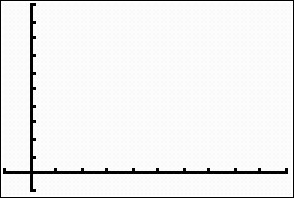
\includegraphics[width=0.4\linewidth]{GraphP1.jpg}
\end{figure}



c. Did the book travel more distance during the push, or while it slid to a stop? Justify answer.

\bigskip
\bigskip
\bigskip
\bigskip
\bigskip
\bigskip
\bigskip
\bigskip

d. There is a moment where the prof lets the book go, and the acceleration changes. The rate of change of the acceleration is called ``jerk" (seriously). Compare the jerk of the book when let go to the jerk of a car accelerating during a freeway merge - which is larger and why? (I'm looking for a clear explanation of your answer). Do you think there is a limit to how large jerk can be? You can speculate here.



\newpage

2. A ball is thrown straight up at $t=0$, rises up until its apex at time $t=T$, comes down, and is caught. 

a. What is the velocity and acceleration at the apex? (We are on Earth.)

\bigskip
\bigskip
\bigskip
\bigskip
\bigskip
\bigskip

b. Consider time $T/2$. Is the ball halfway to its apex, less than halfway, or more, in terms of distance? If you're not sure, draw a graph of its position or velocity vs time. You can ignore air resistance. Justify answer.

\bigskip
\bigskip
\bigskip
\bigskip
\bigskip
\bigskip
\bigskip
\bigskip



c. How do your answers to part (a) change if there is air resistance?

\bigskip
\bigskip
\bigskip
\bigskip
\bigskip
\bigskip
\bigskip



3*.  Consider an air resistance force proportional to $v$, so $F_{air}=-mkv$ for some constant $k$. Write the Newton equation of motion $F=m\frac{dv}{dt}$ for the ball on the way up and then integrate to find the time it takes to reach the apex, if the initial speed of the ball is $v_0$. Compare to the time with no air resistance and show they are equal in the limit of small $k$. What are the units of $k$? What do you think is a characteristic time for this problem?


\end{document}